\section[Exposicion]{C\'alculo de la exposici\'on}

\begin{frame}
 \frametitle{Estrategia de cada b\'usqueda}
 \begin{center}
  \pgfimage[width=0.9\textwidth]{./fig/estrategiaAuger/analysisSchema_4}
 \end{center}
\end{frame}

\begin{frame}
 \frametitle{C\'alculo de la exposici\'on}\footnotesize
 
 \begin{exampleblock}{Definici\'on}
%  \scriptsize
 \begin{displaymath}
 N_{esp}=\int\limits_{\mathbf{E_{\nu}}}~\Phi(E_{\nu}){\cal E}(E_\nu)~dE_\nu
 \end{displaymath}
 \end{exampleblock}

 \begin{block}{Exposici\'on a neutrinos DG}<uncover@2->
 \scriptsize
	\begin{displaymath}
	 {\cal E}_{DG}(E_\nu)\equiv\iint\limits_{\mathbf{D}~\Omega}
	 {\color{Red}
	 P(D|E_{\nu},\omega)~
	 }
	 {\color{Green}
	 \left[~
	 \iint\limits_{T~A}\epsilon(E_{\nu},\omega,D,\vec{r},t)~d\vec{r}~dt
	 \right]
	 }
	 ~d\omega~dD
	\end{displaymath}
 \end{block}
 \begin{block}{Exposici\'on a neutrinos ES}<uncover@2->
 \scriptsize
%   \footnotesize
	\begin{displaymath}
	 {\cal E}_{ES}(E_\nu)\equiv\iiint\limits_{\mathbf{E_\tau}~\mathbf{x_d}~\Omega}
	 {\color{Red}
	 P({\rm x_d},E_\tau|E_{\nu},\omega)~
	 }
	 {\color{Green}
	 \left[~
	 \iint\limits_{T~A}\epsilon(E_\tau,\omega,{\rm x_d},\vec{r},t)~d\vec{r}~dt
	 \right]
	 }
	 ~d\omega~d{\rm x_d}~dE_\tau
	\end{displaymath}
 \end{block}
 
 \begin{block}{Interpretaci\'on}<uncover@3>
	\begin{itemize}
	\item {\color{Red} Probabilidad de iniciar una lluvia dado un neutrino incidente.}
	\item {\color{Green} Cuantas de esas lluvias se esperan haber detectado durante la medici\'on.}
	\end{itemize}
 \end{block}
\end{frame}
% 
\begin{frame}{C\'alculo de los t\'erminos de probabilidad}
\footnotesize
 \begin{block}{Lluvias DG}
  \centering
%   \begin{displaymath}
  $$
   P(D|E_{\nu},\theta) = \frac{1}{m}~\sigma(E_{\nu})\cos\theta
   $$
%   \end{displaymath}
 \end{block}
 
 \begin{block}{Lluvias ES}
  \begin{enumerate}
   \item Espectro de energ\'ia de los $\tau$ que escapan de la tierra $f(E_\tau|E_\nu,\theta)$ obtenido mediante Monte Carlo.
	\begin{center}
		\pgfimage[width=0.45\textwidth]{./fig/exposicionAuger/pdfs_defensa}
	\end{center}
   \item Probabilidad de decaimiento del $\tau$ en la atm\'osfera:
   \begin{displaymath}
    h(x_d,(E_\tau,\theta))=
		\exp{\left(
		-\frac{x_d}{|\cos\theta|\lambda(E_\tau)}
		\right)}
		\frac{1}{|\cos\theta|\lambda(E_\tau)}
   \end{displaymath}
  \end{enumerate}
 \end{block}
\end{frame}
 
% % \begin{frame}
% % \frametitle{C\'alculo de la exposici\'on}
% % 	\begin{textblock}{15}(0.5,2)
% % 		\begin{block}{}
% % 		\footnotesize
% % 		\centering
% % 			$
% % 			\mathcal{E}_{diffuse}(E_{\nu})
% % 			=
% % 			\int\limits_{lifetime} dt
% % 			\int\limits d\Omega
% % 			\int\limits_{minE_\tau^{MC}}^{E_\nu}dE_\tau
% % 			\int\limits_0^\infty dh_{10}
% % 			{\color{red}
% % 			\frac{d^2p_\tau}{dE_\tau d\theta}(E_\tau,h_{10})
% % 			}
% % 			{\color{ForestGreen}
% % 			A_{eff}(E_\tau,\theta,h_{10},t_{conf})
% % 			}
% % 			\times
% % 			\cos\theta
% % 			$
% % 		\end{block}
% % 	\end{textblock}
% % 	
% % 	\begin{textblock}{7.5}(0.5,4)
% % 	\footnotesize
% % 		\begin{alertblock}{Probabilidad iniciar una lluvia:}
% % 			\begin{enumerate}
% % 			\item Probabilidad de que un $\tau$ con $E_\tau$ emerja de la tierra dado un neutrino con $E_\nu$ y $\theta$.
% % 				\begin{itemize}
% % 				\scriptsize
% % 					\item Monte Carlo dedicado.
% % 				\pgfimage[width=\textwidth]{./fig/exposicionAuger/pdfs_defensa}
% % 				\end{itemize}
% % 			\item Convolucionado con la probabilidad de decaer en la atm\'osfera (decaimiento exponencial).
% % 			
% % 			\end{enumerate}
% % 		\end{alertblock}
% % 	\end{textblock}
% % % 	
% % % 	
% % % 	\begin{textblock}{5.8}(6.6,2.5)
% % % 	\scriptsize
% % % 	\visible<2->{		
% % % 		\begin{exampleblock}{Effective Area (Same as in DGH analysis)}
% % % 			\begin{enumerate}
% % % 			\item Choose representative 3-day configuration
% % % 			\item Throw showers of fixed ($E_\tau$, $\theta$,$h_{10}$) inside circular area containing the configuration
% % % 				\begin{center}
% % % 					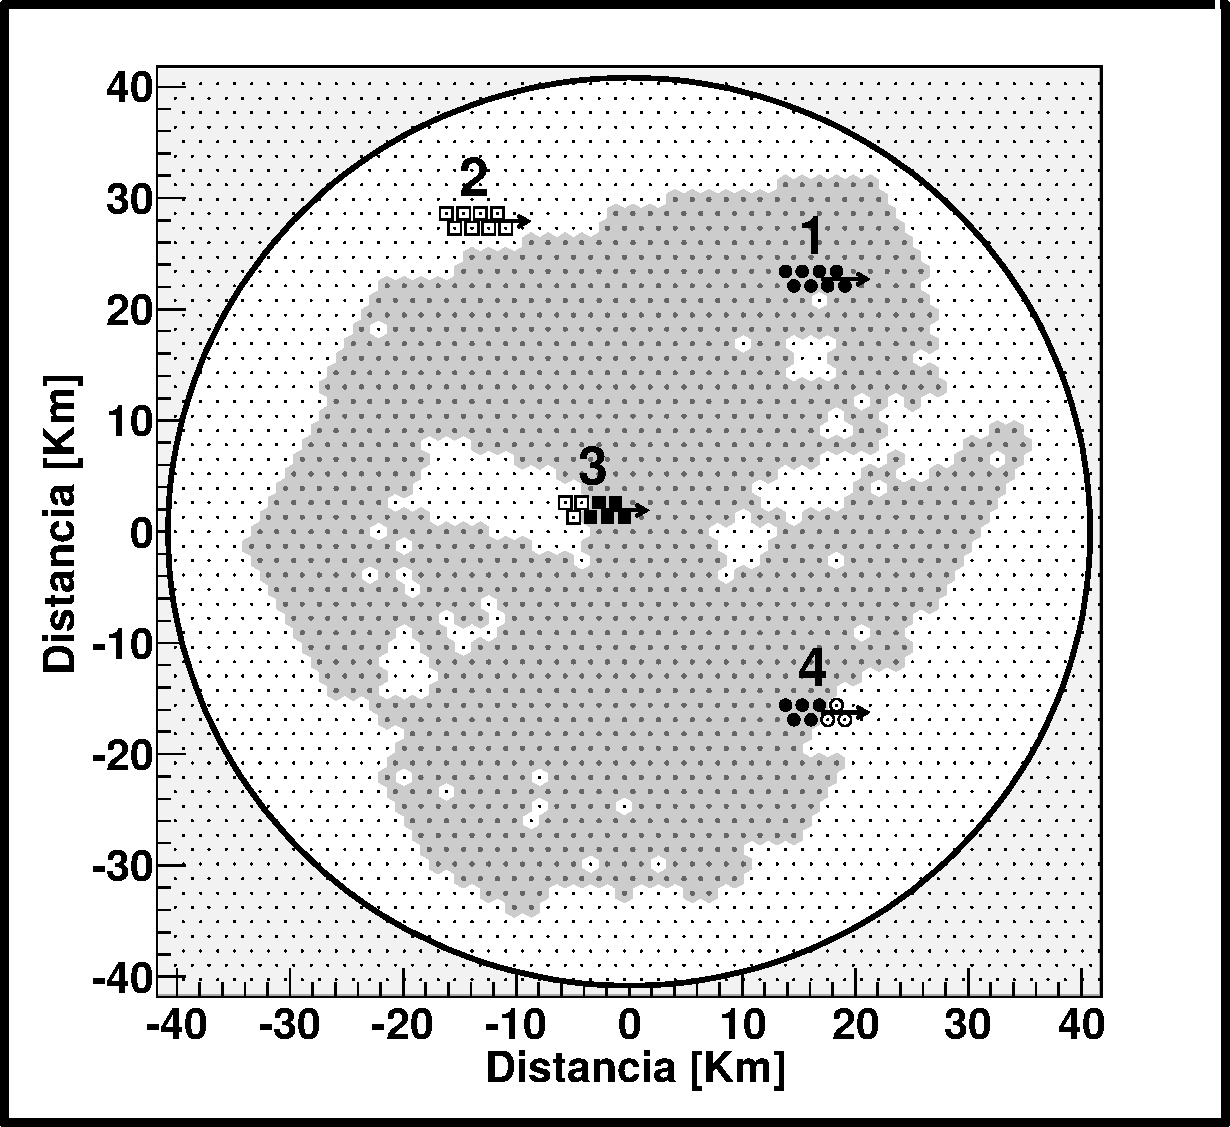
\includegraphics[width=0.5\textwidth]{./fig/aperturaReal.pdf}				                                                            
% % % 				\end{center}
% % % 			\item Apply selection cuts and 
% % % 				\begin{flushright}
% % % 				$\mathcal{A}_{Eff}=\mathcal{A}_{Circ}\times\frac{\nu_{selected}}{\nu_{simulated}}$
% % % 				\end{flushright}
% % % 			\end{enumerate}
% % % 		\end{exampleblock}
% % % 	}
% % % 	\end{textblock}
% % % 	
% % % 	\begin{textblock}{10.7}(1,4)
% % % 	\visible<3->{		
% % % 		\begin{block}{Changes in the three mail ingrediets in the exposure calculation}
% % % % 			\centering
% % % 		\begin{enumerate}
% % % 		\item<3-|alert@3> The calculation method itself $\Rightarrow$ Minor changes in the final result
% % % 		\item<4-|alert@4> The $\nu_\tau$ and $\tau$ interaction models in the Earth
% % % 		\item<5|alert@5> The simulation libraries 
% % % 	\end{enumerate}
% % % % 			\textbf{March 2011 Yann Guardincerri's talk:\\ ``Earth-skimming analysis revisited''}
% % % 		\end{block}
% % % 	}
% % % 	\end{textblock}
% % \end{frame}
% 
% % \begin{frame}{Obtenci\'on de las eficiencias}
% % 	\begin{block}{Las eficiencias dependen de la posi\'on de la lluvia}
% % 		\begin{center}
% % 		\pgfimage[width=0.75\textwidth]{fig/exposicionAuger/lluviaFuera}
% % 		\end{center}
% % 	\end{block}
% % \end{frame}
% 
\begin{frame}{Integraci\'on de las eficiencias}
	\begin{block}{M\'etodo de calculo}
	\begin{enumerate}[<uncover@+-|alert@+>]
	 \item Elegir una configuraci\'on representativa cada 3 dias.
	 \item Lanzar las lluvias sobre tal configuraci\'on y recalcular los criterios de disparo.
	 
	 \begin{center}  
		\visible<2->{\pgfimage[width=0.45\textwidth]{fig/exposicionAuger/aperturaReal}}
	 \end{center}
	 \item Calcular la integral como: $\sum_{t_i} {\cal A}_{circ} \times \frac{\nu_{sel}}{\nu_{sim}} \times \Delta T_i$
	\end{enumerate}

	\end{block}
% 	\begin{alertblock}{M\'etodo de calculo}
% 		\begin{center}
% 		
% 		\end{center}
% 	\end{alertblock}
\end{frame}
% 
% \begin{frame}{Integraci\'on temporal y en superficie}
% 	\begin{block}{Envejecimiento de detector}
% 		\begin{center}
% 		\pgfimage[width=0.75\textwidth]{fig/exposicionAuger/Out_decaytime_main_2005_01}<1>
% 		\pgfimage[width=0.75\textwidth]{fig/exposicionAuger/Out_decaytime_main_2008_01}<2>
% 		\pgfimage[width=0.75\textwidth]{fig/exposicionAuger/Out_decaytime_main_2013_01}<3>
% 		\end{center}
% 	\end{block}
% \end{frame}
% 
% \begin{frame}{Integraci\'on temporal y en superficie}
% 	\begin{block}{Envejecimiento de detector}
% 		\begin{center}
% 		\pgfimage[width=0.9\textwidth]{fig/exposicionAuger/timeEvolution_1}<1>
% 		\pgfimage[width=0.9\textwidth]{fig/exposicionAuger/timeEvolution_2}<2>
% 		\pgfimage[width=0.9\textwidth]{fig/exposicionAuger/timeEvolution_3}<3>
% % 		\pgfimage[width=0.9\textwidth]{fig/exposicionAuger/fractionEvolution}<4>
% 		\end{center}
% 	\end{block}
% \end{frame}
% 
% 
% % \begin{frame}{Integraci\'on temporal y en superficie}
% % 	\begin{block}{Envejecimiento de detector}
% % 		\begin{center}
% % 		\pgfimage[width=0.55\textwidth]{fig/exposicionAuger/timedecay_vs_reflect_absorp_2}
% % 		\end{center}
% % 	\end{block}
% % 	\begin{block}{Envejecimiento de detector}<2>
% % 		\begin{center}
% % 		\renewcommand{\arraystretch}{1.4}
% % 		\footnotesize
% % 		\begin{tabular}{|l|ccc|c|}
% % 					\hline
% % 					Período       & tyRef & wAbs & LDT        &    Pérdida de exposición \\
% % 					\hline
% % 					$2004 - 2008$ & 0.94  & 100  & $\sim63$ns &    $--$ \\
% % 					$2009 - 2010$ & 0.94  & 80   & $\sim60$ns &    $-15.2\%$\\
% % 					$2011 - 2013$ & 0.93  & 100  & $\sim57$ns &    $-17.5\%$\\
% % 					\hline
% % 		\end{tabular}
% % 		\end{center}
% % 	\end{block}
% % \end{frame}
% 
% 
\begin{frame}{Exposici\'on combinada}
	\begin{alertblock}{}
		\begin{center}
			\textbf{La muestra de datos es escrutada con los tres criterios}
		\end{center}
	\end{alertblock}
	\begin{block}{M\'etodo de combinaci\'on}
		\begin{center}
		\pgfimage[width=0.75\textwidth]{fig/exposicionAuger/sketch_combined_5}
		\end{center}
	\end{block}
\end{frame}
% 
\begin{frame}{Exposici\'on combinada}
	\begin{block}{Obtenci\'on de la exposicion total}
		\begin{center}
			\begin{displaymath}\renewcommand{\arraystretch}{2}
			\begin{array}{rcl}
			N_{esp}& =& N_{esp}^{DGL}+N_{esp}^{DGH}+N_{esp}^{ES} \\ 
			& = & \int\limits_{E_\nu}\Phi(E_\nu)~({\cal E}^{DGL}+{\cal E}^{DGH}+{\cal E}^{ES})(E_\nu)~dE_\nu\\
			& \equiv & \int\limits_{E_\nu}\Phi(E_\nu)~{\cal E}(E_\nu)~dE_\nu
			\end{array}
			\end{displaymath}
		\end{center}
	\end{block}
	
	\begin{alertblock}{}
	\centering
% 		\begin{center}
			\begin{displaymath}
			{\cal E}(E_\nu) = {\cal E}^{DGL}+{\cal E}^{DGH}+{\cal E}^{ES}
			\end{displaymath}
% 		\end{center}
	\end{alertblock}
	
	\begin{exampleblock}{}
		\begin{center}
			\textbf{La exposici\'on combinada es la suma de las individuales}
		\end{center}
	\end{exampleblock}
\end{frame}

\begin{frame}{Exposici\'on combinada}
	\begin{block}{Resultado}
		\begin{center}
		\pgfimage[width=0.75\textwidth]{fig/exposicionAuger/exposure_combined_ageing}
		\end{center}
	\end{block}
	\begin{alertblock}{}
		\begin{center}
			\textbf{El canal ES domina a bajas ener\'ias}
		\end{center}
	\end{alertblock}
\end{frame}
% 
\begin{frame}{Exposici\'on combinada}
	\begin{block}{Distribuci\'on de la exposici\'on}
		\begin{center}
		\begin{tabular}{|c|c|c|c|c|}
			\hline
			\diagbox{Lluvia}{Criterio} & ES & DGH & DGL  & Total\\ \hline
			ES     &    0.80       &    0.04       &     $<0.001$ & 0.84 \\ \hline
			DGH    &    0.03       &    0.11       &     $<0.001$ & 0.14 \\ \hline
			DGL    &    $<0.001$   &    $<0.001$   &     0.02     & 0.02 \\
			\hline
		\end{tabular}
		\end{center}
	\end{block}
	\begin{alertblock}{Matriz de clasificaci\'on}<uncover@2>
		\begin{center}
		\begin{tabular}{|c|c|c|c|c|c|}
			\hline
			\diagbox{Lluvia}{Criterio} & ES $\wedge$ DGH &  ES    &  DGH   &  DGL      \\ \hline
			ES                         & 0.90            &  0.86  &  0.48  &  0.00     \\ \hline
			DGH                        & 0.10            &  0.14  &  0.52  &  0.03     \\ \hline
			DGL                        & 0.00            &  0.00  &  0.00  &  0.97     \\ \hline\hline
			Probabilidad               & 0.69            &  0.20  &  0.09  &  0.02     \\
			\hline
		\end{tabular}
		\end{center}
	\end{alertblock}
\end{frame}
% 
\begin{frame}{Errores sistem\'aticos}
	\begin{block}{Errores sistem\'aticos}
		\begin{center}
			\renewcommand{\arraystretch}{1.4}
			\scriptsize
% 			\newcolumntype{C}[1]{>{\centering\arraybackslash}p{#1}}
				\begin{tabular}{|C{0.2\textwidth}|c|c|c|c|}
% 				\begin{tabular}{|l|c|c|c|c|}
				\hline
				Fuente del  & ES        & DGH       & DGL        & Combinaci\'on         \\
				sistemático & ($90^\circ,95^\circ$) & ($75^\circ,90^\circ$) & ($65^\circ,75^\circ$) & ES / DGH / DGL   \\
		% 		\hline
		% 		& {\tiny \bf GAP 2013-100}     & \multirow{2}{*}{\tiny \bf PRD 84, 2011}    &   \multirow{2}{*}{\tiny \bf GAP2013-013} & \multirow{2}{*}{\tiny \bf 83.9\% / 13.7\% / 2.4\% }\\
		% 		& {\tiny \bf PRD 79, 2009}     &     &  &  \\
				\hline
				
				Gen. de interacción primaria    &  no apl. &   0\%, -7\%     &   +3\%, -4\%  & +0.07\%, -1.0\% \\
				
				\hline
				
				PDF en el generador             &  no apl. &   0\%, -7\%     &   +4\%, -5\%  & +0.1\%, -1.0\% \\
				
				\hline
				
				Simulador de EAS                &  no eval. &   0\%, -17\%    &   +17\%, 0\%  & +0.4\%, -2.3\% \\
				
				\hline
				
				Modelo hadrónico                & +4.7\%, -1\%      &  +5\%, -2\%     &   +0\%, -6\%  & +4.6\%, -1.3\% \\
				
				\hline
				Algoritmo de thinning           & +0.3\%, 0\%   &  +7\%,  0\%     &   +7\%,  0\%  & +1.1\%, -0.0\% \\
				\hline
				\hline
				\multirow{2}{*}{\bf $\bm{ \sigma_{\nu_\tau}\ \otimes\ \tau}$ E-loss}    & \multirow{2}{*}{\textcolor{Red}{+40\%, -33\%}}  & \multirow{2}{*}{+9\%, -9\%}  & \multirow{2}{*}{+7\%, -7\%} & \multirow{2}{*}{\bf +35\%, -29\%} \\
													&                 &                 &             & \\
				\hline
				\hline
		% 				%%%%%%%%%%%%%%%%%%%%%%%%%%%%%%%%%%%%%%%%%%%%%%%%%%%%%%%%%%%%%%%%%%%%%%%%%%%%%%%%%%%%%%%%%%%%%%%%%%
				Topography          &  +18\%, 0\%    & +24\%, 0\% & not apl.   & +18\%, 0\%  \\
				\hline
				\hline
				{\bf Total}                     &  \multicolumn{3}{c|} {}  & {\bf +39\%, -29\%}         \\
				\hline
				%%%%%%%%%%%%%%%%%%%%%%%%%%%%%%%%%%%%%%%%%%%%%%%%%%%%%%%%%%%%%%%%%%%%%%%%%%%%%%%%%%%%%%%%%%%%%%%%%%
				\end{tabular}
		\end{center}
	\end{block}
	\begin{exampleblock}{}
		\begin{center}\footnotesize
			La combinaci\'on se obtuvo teniendo en cuenta la contribuci\'on relativa de cada canal a la exposici\'on.
		\end{center}
	\end{exampleblock}
\end{frame}